\section{Introduction}
\label{sec:intro}

Fine-grained image recognition (FGIR) distinguishes visually similar subcategories, such as bird species or car models~\cite{wah2011cub,krause2013cars}.
Ultra-fine-grained recognition extends this task to cultivars, such as soybean and cotton varieties that experts struggle to tell apart~\cite{yu2021benchmark,fang2024learning}.
Accuracy on these tasks improves with larger backbones \TBD{citation for the accuracy gain of larger backbones on FGIR}.
However, larger backbones need more memory and computation, which limits their use on edge devices.
Quantization reduces this cost by representing weights, and possibly activations, at lower numerical precision.

Quantization-aware training (QAT) adapts the model parameters to reduced precision during training, and usually reaches higher accuracy.
However, it requires an additional training stage and suitable training data.
Post-training quantization (PTQ) instead converts an already trained model without a full training stage, with at most a small calibration set~\cite{gholami2021survey}.
Half-quadratic quantization (HQQ) needs no calibration data at all~\cite{badri2023hqq}.
PTQ therefore offers a fast way to reduce the model size when training resources or the original data are limited, while keeping acceptable accuracy.

Much research improves the accuracy of PTQ.
For vision transformers, PTQ4ViT handles difficult activation distributions through twin uniform quantization and Hessian-guided calibration~\cite{yuan2022ptq4vit}.
Mixed-precision methods such as LampQ allocate bit widths according to the sensitivity of each component~\cite{kim2026lampq}, and data-limited methods synthesize calibration data~\cite{zhong2022fdda,kim2025synq}.
Other work shows that the accuracy loss is uneven.
In medical imaging, it varies across datasets and backbones~\cite{ozdemir2026bridging}.
Classes and population groups can also degrade unequally~\cite{liu2025unfairness}, and the worst-case group depends on the calibration distribution~\cite{yuan2023benchmarking}.
At the sample level, prediction changes after quantization have been associated with small output margins~\cite{hu2023towards}.
These findings suggest that, under the same model and quantization setting, the accuracy retained can still differ between datasets.
This leads to our first question: does the dataset affect quantization robustness?

\begin{figure}[t]
  \centering
  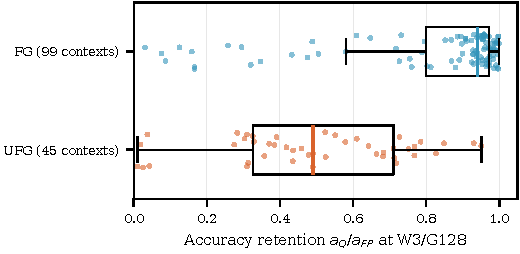
\includegraphics[width=\linewidth]{figures/retention_box.pdf}
  \caption{Accuracy retention at 3-bit weights with group size 128 for every context, one point per dataset, backbone and fine-tuning strategy. UFG: the five soybean and cotton cultivar datasets. FG: the other fine-grained datasets.}
  \label{fig:teaser}
\end{figure}

To answer it, we quantize three backbones, each trained with three fine-tuning strategies on \V{nDatasets} datasets, at \V{nBits} bit widths and \V{nGroupSizes} group sizes, and compare every quantized model with its own unquantized checkpoint.
\cref{fig:teaser} shows a clear difference between two kinds of datasets.
At 3-bit weights, each of the five ultra-fine-grained (UFG) cultivar datasets keeps at most \V{maxSc_w3g128} of its accuracy on average, while each fine-grained (FG) dataset keeps at least \V{minOther_w3g128}.
However, the UFG datasets also have much lower baseline accuracy, so the difference alone does not say which property of the data matters.
This leads to our second question: how and why does the dataset affect quantization robustness?
To address it, we test whether the ranking of datasets holds across quantization conditions, backbones and strategies, and whether the baseline decision margins account for the difficulty beyond baseline accuracy.
We then reweight the test images of the two groups to equal margin distributions, and compare the features and decisions of the baseline and quantized models.
Our contributions are as follows:
\begin{enumerate}
  \item We show that the dataset affects quantization robustness: in every backbone and fine-tuning strategy, the UFG datasets lose more accuracy than the FG datasets where retention lies between collapse and full retention, and the separation of the two groups is stable while the order within the FG group is not.
  \item We show that the baseline logit margin correlates with the difficulty at least as strongly as any other measured property, including baseline accuracy, and separates some datasets that baseline accuracy cannot; matching it narrows the gap between the groups by about half, while feature similarity does not track the loss.
\end{enumerate}
